\chapter{Macros para Excel}

\section{Principios de Macros}


\subsection{Grabación de macros}

Excel permite la grabación de ciertos pasos y procedimientos que se hagan en la hoja de excel, para guardarlos como procedimientos automáticos que se pueden repetir en el futuro. El \textit{shortcut} \texttt{alt + T + M + R} permite abrir el cuadro de grabación de macro. 

Se puede asignar un atajo de teclado, si se pone en mayúscula queda \texttt{alt + Mayus + ...}. 

El código que se genera o se escribe se guarda generalmente dentro de la carpeta \textit{Modules}, si es un codigo que aplica al libro de trabajo entero. Y el código que es específico para una hoja en particular se guarda o permanece dentro de esa misma hoja. \\

Alternando la opción de referencias relativas se puede realizar grabaciones para elementos como tablas dinámicas.

En la pestaña \textit{Development-Insert} se pueden agregar controles de ejecución de macros.


\subsection{Fundamentos de Visual Basic}

\subsubsection{\texttt{Sub} Procedimientos}

La gran mayoría de procedimientos que se escribirán dentro de una macro está dentro del \textbf{sub} procedimiento

\begin{verbatim}
Sub my_Macro()

End Sub
\end{verbatim}

\subsubsection{Procedimientos de \texttt{funciones}}

Esta es una forma de escribir y definir fórmulas propias (tienen un valor de retorno). Pueden ser usadas en celdas de excel. También se usa para retornar valores a los sub procedimientos.

\begin{verbatim}
Function my_Formula()

End Function
\end{verbatim}

\subsubsection{Colores}

\paragraph{Azul} Se asigna a algunas de las palabras reservadas. Las palabras reservadas inician con letra mayúscula, aunque no es necesario escribirlas de tal forma porque el editor las pone de fomra automática.

\paragraph{Rojo} Indica error de sintaxis


\paragraph{Verde} Los comentarios vienen en ese color

\paragraph{Salto de línea} El salto de línea que se realiza cuando esta es muy larga se hace de la forma siguiente


\begin{verbatim}
Selection.Borders(xlDiagonalUp._
LineStyle = xlNone
\end{verbatim}


\subsubsection{Algunos atajos de teclado}

\begin{table}[H]
    \centering
    \begin{tabular}{|c||c|}
        \hline
        Descripción & Tecla \\ \hline
        Abrir buscador de objetos & \textbf{F2} \\ \hline
        Abrir ventana de código & \textbf{F7} \\ \hline
        Mostrar ventana de propiedades & \textbf{F4} \\ \hline
        Ejecutar proyecto & \textbf{F5} \\ \hline
        Pasar al código & \textbf{F8} \\ \hline
    \end{tabular}
    \caption{Caption}
    \label{tab:my_label}
\end{table}

\subsection{El modelo Objeto}

Una forma de hacer referencia (instancia) a un objeto \texttt{Range}, por ejemplo la celda "A1" es la siguiente

\begin{verbatim}
Application.Workbooks("Name").Worksheets("WSname").Range("A1")
\end{verbatim}

\texttt{ThisWorkbook} es una referencia al libro de trabajo sobre el cual se está escribiendo el código, para referenciarse a sí mismo. Cuando se omite la instancia a un objeto, se asume que es el "más cercano" o el que está activo actualmente. Por ejemplo \texttt{Range("A1")} asume que se trata de la hoja de trabajo activa. \texttt{ActiveCell} asume la celda marcada en la hoja de trabajo activa.

\subsubsection{Propiedades y métodos de los objetos}

\texttt{Range("A1").Address} o \texttt{Range("A1").Value} son ejemplos de atributos o propiedades que no tienen detalles. Por el contrario, \texttt{Range("A1").Interior.Color} o \texttt{Range("A1").Font.Color} hacen referencia al atributo \texttt{Color} pero de objetos diferentes: "fuente" e "interior". \\

La propiedad \texttt{Range("A1").Interior} tiene como retorno un objeto \texttt{Inerior}. Muchas propiedades pueden ser solo de lectura o de lectura y escritura. Es decir, se puede asignar un atributo.

\subsubsection{Métodos}

Muchos métodos no necesitan argumentos, para los que sí necesitan, la forma de especificarlos es mediante un espacio:

\begin{verbatim}
Range("A2").Delete xlShiftToLeft
Range("A2").Copy Range("B2")
Range("C3").PasteSpecial xlPasteValues
\end{verbatim}

Cuando un método tiene más de un argumento opcional, y solo se requiere especificar el segundo u otro que no es el primero, se pude usar de la siguiente forma

\begin{verbatim}
Sheet1.Copy After:=Sheet3
Sheet1.Copy , Sheet2
\end{verbatim}

En la primera línea del código anterior, se especifica el argumento que quiero ingresar; en la segunda línea se indica que estoy poniendo el segundo argumento.

\subsubsection{Cómo encontrar los atributos o métodos necesarios}

Una forma de verificar el nombre de un objeto, método o atributo es mediante la grabación de macros. Se puede buscar también en la librería de objetos (\textbf{F2}) y con el botón de ayuda (\textbf{F1}) para encontrar la documentación. Otra manera es mediante el despliegue de opciones (\textbf{Ctrl + Space}).

\textit{\textbf{Clase 21 del curso, se explica cómo obtaner ayuda del immediate}}

 \paragraph{Ejemplo} Para el objeto \texttt{Comment} se tienen los siguientes atributos y métodos:
 
 \begin{figure}[H]
     \centering
     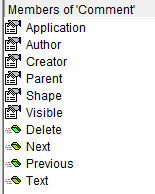
\includegraphics{ExcelMacro/commentobj.png}
 \end{figure}
 
Desde \texttt{Application} hasta \texttt{Visible} son los atributos y desde \texttt{Delete} hasta \texttt{Text} se tienen los métodos.

Si hay un comentario en la celda \textit{F6}, el objeto \texttt{Range("F6")} tiene como atributo \texttt{Comment} (\texttt{range("F6").Comment}) 

\begin{figure}[H]
    \centering
    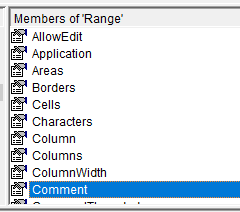
\includegraphics{ExcelMacro/rangeatr.png}
\end{figure}

Por tanto, el objeto \texttt{Comment} tendrá como atributo \texttt{Parent} esa celda:


\begin{verbatim}
?activesheet.Comments(1).Parent.Address
$F$6
\end{verbatim}

\subsubsection{Resumen y conclusiones}

\begin{enumerate}
    \item Para referenciar un objeto se hace a través de su posición en la jerarquía del objeto. El objeto activo es el objeto que está referenciado actualmente; si uno no especifica el objeto padre de una referencia, Excel asumirá que se trata del objeto activo.
    \item No es necesario seleccionar un objeto para manipularlo; aunque existe el método \texttt{Select}, en la práctica no se usa y es más eficiente evitar su uso (aunque hay algunas excepciones) 
\end{enumerate}


\subsection{Referencias a rangos, hojas y libros de Excel con VBA}

El objeto \texttt{Range} es uno de los más importantes y usados en los macros, por lo tanto es importante entender bien y saber cuáles son los métodos y atributos más usados. También cómo se pueden referenciar de forma correcta las diferentes hojas o libros de excel. 

\subsubsection{Métodos de escritura en celdas}

\paragraph{Recordatorio} Diferencia entre los atributos \texttt{Activecell} y \texttt{Selection}, cuando se tiene seleccionadas las celdas \textit{M7:M14}
    \begin{verbatim}
    ?activecell.Address
    $M$7
    ?selection.Address
    $M$7:$M$14
    $K$5
    \end{verbatim}

La siguiente lista muestra cómo referenciar un rango de distintas formas.

\begin{itemize}
    \item \texttt{Range().Value = "1st"} 
    \item \texttt{Range(R1,R2).Value = "hola"} Pone el valor en todas las celdas desde R1 hasta R2. 
    \item \texttt{Range("R1;R2").Value = "hola"} Pone el valor solo en las referencias especificadas R1 y R2
    \item \texttt{Activecell.Value="Otrooo"} Valor en la celda actualmente activa
    \item \texttt{Range("A" \& 6, "J" \& 27) = "6th"} Utiliza índice numérico que puede ser iterado en bucles. Escribe "6th" en las celdas desde A6 hasta J27.
    \item \texttt{Range(Cells(1, 6), Cells(10, 20)) = "6th"} Para referenciar numéricamente un rango y pueda ser implementado en bucles o iteraciones.
    \item \texttt{Range("A1").Offset(7,2).Value = ...} Se ubica en A1 y busca a partir de ahí el movimiento (7,2) para ubicar el valor en esa casilla. 
    \item \texttt{Range("Reference").Value = "Puting here a reference"} Si se le cambia el nombre a una celda como indica la imagen de abajo, se puede referenciar con ese nombre.
    \item \texttt{Rows("12:14").RowHeight = 35} cambia el tamaño de las filas 12 hasta 14.
    \item \texttt{Columns("W:AA").ColumnWidth = 5} cambia el tamaño de las columnas W hasta AA.
    \item \texttt{Range(Columns(7), Columns(10)).ColumnWidth = 5} Tamaño de las columnas desde la 7ma  columna hasta la 10ma usando Range.
    \item \texttt{Range(Rows(7), Rows(10)).RowHeight = 25} Tamaño de las filas desde la 7ma  columna hasta la 10ma usando Range.
    \item \texttt{Cells.Columns.AutoFit} pone tamaño minimo de todas las columnas
\end{itemize}


\begin{figure}[H]
    \centering
    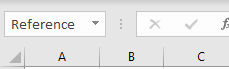
\includegraphics{ExcelMacro/reference.png}
\end{figure}

\subsection{Métodos y atributos más usados e importantes del objeto Range}

Los atributos y métodos más útiles que son necesarios saber y tener en cuenta cómo se trabajan en VBA.

\begin{table}[H]
    \centering
    \begin{tabular}{|m{0.15\columnwidth}|m{0.60\columnwidth}|m{0.1\columnwidth}|}
        \hline
        \rowcolor{lightgray} \textbf{Atributo} & \textbf{Descripción} & \textbf{Tipo} \\ \hline \hline
        \texttt{Value}        & Valor que está escrito en la celda. Es la propiedad por defecto & Lect/Esc \\ \hline
        \texttt{Cells}        & Retorna una celda o un rango de celdas dentro del rango  & Lect/Esc  \\ \hline
        \texttt{End}          & Retorna la última celda del rango. Similar a Ctrl + up, down, left o right. Recibe como argumento una de las cuatro direcciones: \texttt{xlDown, xlToLeft, xlToRight, xlUp} & Solo Lect  \\ \hline
        \texttt{Offset}       & Retorna la celda que está referenciada desde el lugar de origen, cierto número de filas o columnas.  & Lect/Esc  \\ \hline
        \texttt{Count}        & Retorna el número de celdas que hay en el rango  & Solo Lect  \\ \hline
        \texttt{Column/Row}   & Retorna el índice de la fila o columna del rango. Si el rango es de más de una celda, rel retorno es el primero de ellos.  & Solo Lect  \\ \hline
        \texttt{CurrentRegion}& Retorna las celdas o rango que pertenecen a una región de datos.  & Solo Lect  \\ \hline
        \texttt{EntireColumn}/
        \texttt{EntireRow}    & Retorna el rango con todas las celdas de la columna o fila  & Solo Lect \\ \hline
        \texttt{Resize}       & Cambia el tamaño del rango definiendo las filas y columnas para reescalado  & Solo Lect  \\ \hline
        \texttt{Address}      & Retorna la dirección de la celda  & Solo Lect  \\ \hline
        \texttt{Font}         & Retorna el objeto Fuente perteneciente a la celda  & Lect/Esc  \\ \hline
        \texttt{interior}     & Es el relleno o interior de la celda. Tiene sus propios atributos como color y demás  & Lect/Esc  \\ \hline
        \texttt{Formula}      & Escribe una fórmula en la celda(s)   & Lect/Esc  \\ \hline
        \texttt{NumberFormat} & Define el formato numérico de la(s) celda(s)   & Lect/Esc  \\ \hline
        \texttt{Text}         & Retorna el dato que haya en la celda como un string   & Solo Lect  \\ \hline
        \texttt{HasFormula}   & Retorna un valor de verdad o \texttt{Null} si son varias celdas y tiene ambos valores de verdad   & Solo Lect  \\ \hline
    \end{tabular}
    \caption{Diferentes atributos útiles}
    \label{tab_rangea}
\end{table}



\begin{table}[H]
    \centering
    \begin{tabular}{|m{0.15\columnwidth}|m{0.60\columnwidth}|}
        \hline
        \rowcolor{lightgray} \textbf{Método} & \textbf{Descripción} \\ \hline \hline
        \texttt{Copy}         & Es práctico porque tiene su destino como argumento, permitiendo copiar y pegar en una sola línea \\ \hline
        \texttt{PasteSpecial} & Permite las opciones de excel de pegado especial. Para usar más de una opción se repite la línea de código con las nuevas opciones \\ \hline
        \texttt{Clear}        & Borra el contenido y el formato de las celdas  \\ \hline
        \texttt{Delete}       & Borra las celdas y realiza in corrimiento de las celdas adyacentes. Es necesario poner argumentos para el corrimiento de la información   \\ \hline
        \texttt{SpecialCells} & Retorna un rango que coincida con los tipos de celda especificado \\ \hline
        \texttt{Sort}         & Ordena un rango de valores.   \\ \hline
        \texttt{PrintOut}     & Se puede usar para imprimir una hoja. \\ \hline
        \texttt{Select}       & Se usa para seleccionar una celda o un rango de celdas. No es necesario usarlo cuando se hace código en VBA, porque no es necesario seleccionar una celda para manipularla.  \\ \hline
    \end{tabular}
    \caption{Diferentes métodos útiles}
    \label{tab_rangem}
\end{table}

\paragraph{Nota} Puede ser útil, para seleccionar o referenciar la última celda de un rango, si en el rango hay bahías, seleccionar desde abajo, siempre y cuando se tenga cereza que no hay ningún valor más abajo, de la siguiente forma

\begin{verbatim}
Range("K6").Value = Range("A" & Rows.Count).End(xlUp).Row
\end{verbatim}

Con \texttt{"A" \& Rows.Count} se está referenciando la última celda de la columna A.

\subsubsection{Copia y pegado de rangos}


\begin{verbatim}
Sub CopyPaste()
    '--------------
    'Mediante el metodo Copy
    '--------------
    Range("A5").CurrentRegion.Copy Range("J4")
    
    '--------------
    'Mediante el metodo PasteSpecial
    '--------------
    Range("A5").CurrentRegion.Copy
    Range("j20").PasteSpecial xlPasteValues
    Range("j20").PasteSpecial xlPasteComments

    '--------------
    'Mediante el propiedad Resize, para copiar contenido sin header
    '--------------
    Range("A5").CurrentRegion.Offset(1, 0).Resize(Range("A5").CurrentRegion.Rows.Count - 1).Copy
    Range("A20").PasteSpecial xlPasteFormulasAndNumberFormats
    Application.DataEntryMode = False
End Sub
\end{verbatim}

\subsubsection{Referenciando Hojas de excel}

Para que uno pueda referenciar la hoja activa mediante el Intellisense, es necesario declarar la hoja como variable

\begin{verbatim}
Dim Sh As Worksheet
Set Sh = ActiveSheet
\end{verbatim}

De este modo se puede usar el Intellisense con el ctrl + espacio. \\

Las hojas de un libro de excel pueden ser referenciadas con su índice (que empieza por 1).

\begin{verbatim}
Worksheets(6).Select
Sheets(6).Select
Worksheets("Purpose").Select
\end{verbatim}

Aquí "\texttt{sheets}" también puede hacer referencia a hojas que no sean de cálculo como \texttt{chart sheets}. Evidentemente se puede referenciar con el nombre de la hoja. Otra manera es mediante el nombre código de la hoja, este se puede ver en la imagen a continuación


\begin{figure}[H]
    \centering
    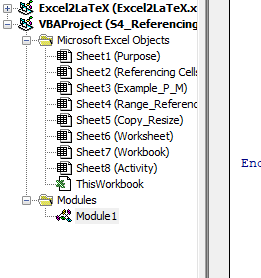
\includegraphics{ExcelMacro/codesheets.png}
\end{figure}

Teniendo en cuenta la imagen, el código sería

\begin{verbatim}
Sheet6.Select
\end{verbatim}

El nombre código de una hoja se puede cambiar.

\subsubsection{Macro que guarda una copia del contenido de un libro}

\begin{verbatim}
ThisWorkbook.Save
Sheets.Select
Cells.Copy
Cells.PasteSpecial xlPasteValues

Application.DisplayAlerts = False

ThisWorkbook.SaveAs Filename:=ThisWorkbook.Path & 
"HC_" & VBA.Format(VBA.Date, "YYMMDD") & "_" & VBA.Replace(ThisWorkbook.Name, ".xlsm", ""),
FileFormat:= Excel.clOpenXMLWorkbook
Application.DisplayAlerts = True

\end{verbatim}

\subsection{Variables y tipos de datos}

Declaración de asignación:
\begin{verbatim}
Range("A1").Value = Date
Range("A1").Value = Range("A1").Value + 1
\end{verbatim}

Para declarar una variable

\begin{verbatim}
myTitle = Range("a8").Value
\end{verbatim}

Los tipos de datos se muestran en la siguiente tabla

\begin{table}[H]
    \centering
    \begin{tabular}{lll}
    \hline
        \textbf{Tipo} & \textbf{Uso de memoria} & \textbf{Rango} \\ \hline
        \rowcolor{micolor1} Byte & 1 byte & 1 a 255 \\ 
        \rowcolor{micolor2} Integer  & 2 bytes & -32768 a 32768 \\
        \rowcolor{micolor1} Long     & 4 bytes & -2147483648 a 2147483648 \\
        \rowcolor{micolor2} Boolean  & 2 bytes & True / False \\
        \rowcolor{micolor1} Double   & 8 bytes & Rango muy grande positivo o negativo con alta precisión \\
        \rowcolor{micolor2} String   & 1 byte por caracter & Depende de la longitud \\
        \rowcolor{micolor1} Object   & 4 bytes & Cualquier objeto \\
        \rowcolor{micolor2} Date     & 8 bytes & 01/01/0100 hasta 12/31/9999 \\
        \rowcolor{micolor1} Currency & 8 bytes & Rango muy grande positivo o negativo hasta 4 decimales \\
        \rowcolor{micolor2} Variant  & 16 bytes o más & Cualquiera, puede ser Vacío, Nada, o Null \\ 
    \end{tabular}
\end{table}

La palabra reservada para declaración de variables es \texttt{Dim}. Una nota importante es que si no se usa la palabra reservada
\texttt{As}, entonces se interpretará el tipo de objeto como \texttt{Variant}.

\begin{verbatim}
Dim myText As String
\end{verbatim}


\paragraph{Nota} se puede usar la palabra reservada \texttt{Debug.Print} para imprimir en consola la variable que se necesite.

\subsubsection{Arrelgos}

Los arreglos (\texttt{Array}) son grupos de variables los cuales tienen el mismo nombre asociado.


Declaración de arreglos

\begin{verbatim}
Dim MyMonth(1 To 12) As String
MyMonth(1) = "Jan"
.
.
.
\end{verbatim}

Si se declara un arreglo de la siguiente forma \texttt{Dim MyMonth(11) As String} se asume el primer índice del arreglo como cero.

Areglos de dos dimensiones:

\begin{verbatim}
Dim MonthSales(1 To 12, 1 To 3) As Variant
Dim MonthSales() As Variant
\end{verbatim}

La última declaración, en la que no hay números en los paréntesis, es un arreglo con tamaño variable.

Para declaración de constantes

\begin{verbatim}
Const MYSCCENARIO As String = "Actual"
\end{verbatim}


Ejempplo de declaración de variables del tipo Objetos


\begin{verbatim}
Dim NewBook As Workbook
Dim NewSheet As Worksheet
Dim NewRange As Range

Set NewBook = Workbooks.Add
\end{verbatim}

\subsubsection{\texttt{scope}}

El scope es es el entorno o subentorno en el que las variables existen, puede ser un sub procedimiento o en todos los sub procedimientos. Las variables solamente existen cuando el procedimiento se está ejecutando. El entorno más pequeño es el entorno de procedimiento. La memoria se libera una vez el procedimiento termina. Un entorno mayor permite declaración de variables que están disponibles en el módulo entero En este caso el \texttt{Dim} está por fuera de cualquier \texttt{Sub}. El valor almacenado permanece en la memoria después de que se ejecuten los procedimientos.

El entorno mayor es aquel en el que se pueden declarar variables para todos los módulos y procedimientos. La palabra reservada para declarar estas variables globales es la siguiente

\begin{verbatim}
Option Explicit
Public LastRow As Long, FirstRow As Long
\end{verbatim}


\subsection{Bucles y ciclos}

\subsubsection{Colecciones}

Las colecciones son conjuntos ordenados de objetos, y pueden ser referenciados como una sola unidad. 

\subsubsection{Secuencia \texttt{With}}

Se usa para hacer un uso más sencillo de código, escribir código más rápido, y para un mantenimiento más fácil. Adicionalmente el código se ejecuta de forma más rápida.

Veamos el siguiente ejemplo

\begin{verbatim}
Set myRange = Range("A10","A" & Cells(Rows.Count, 1).End(xlUp).Row)
myRange.Font.Name = "Arial"
myRange.Font.Size = 12
myRange.Font.Bold = True
\end{verbatim}

Con el adjuntador podemos convertirlo a 

\begin{verbatim}
Set myRange = Range("A10","A" & Cells(Rows.Count, 1).End(xlUp).Row)
With myRange.Font
    .Name = "Arial"
    .Size = 12
    .Bold = True
End With
\end{verbatim}

\subsubsection{Bucle \texttt{For...Each}}


Realiza un iteración del tipo que se escoja dentro de una colección

\begin{verbatim}
Dim Cell As Range
For Each Cell In ActiveSheet.UsedRange
    'Instructions
Next Cell
\end{verbatim}

El siguiente ejemplo es para proteger cada una de las hojas de nuestro cuaderno de excel:

\begin{verbatim}

Sub Protect_All_Sheets()
    Dim Sh As Worksheet
    For Each Sh In ThisWorkbook.Worksheets
        Sh.Protect Password:= "prueba", AllowFormattingCells:= True
        Debug.Print Sh.Name
    Next Sh
    
End Sub

Sub Unprotect_All_Sheets()
    Dim Sh As Worksheet
    For Each Sh In ThisWorkbook.Worksheets
        Sh.Unprotect
        Debug.Print Sh.Name
    Next Sh
    
End Sub
\end{verbatim}

El método \texttt{Protect} tiene varios argumentos, entre los que están \texttt{Password:= "prueba", AllowFormattingCells:= True}, poniendo una contraseña y permitiendo que se cambie el formato de las celdas.

Una forma de proteger el macro con código es mediante \texttt{tools, VBAProject Properties, Protection}.

\subsubsection{\texttt{If...Then}}

El condicional if de toda la vida, es similar a la fórmula de excel y se construye de la siguiente manera

\begin{verbatim}
Sub Simple_if()
    If Range("B3").Value <> "" Then Tange("C3").Value = Range("B3").Value
End Sub    
\end{verbatim}

Con el comparador \texttt{<> ""} se evalúa si la celda en cuestión no está vacía, es decir, si tiene contenido.

\begin{verbatim}
Sub Simple_if()
    If Range("B3").Value <> "" Then 
        Range("C3").Value = Range("B3").Value
    End If
End Sub    
\end{verbatim}

Estructura general de If Else

\begin{verbatim}
If <Comparision> Then
    <Code>
    <Code>
    <Code>
Elseif <Comparision> Then
    <Code>
    <Code>
    <Code>
Else
    <Code>
    <Code>
    <Code>
End If
\end{verbatim}


\subsubsection{\textbf{Case}}

La estructura principal es

\begin{verbatim}
Sub CaseStat()
    Select Case Range("B3").Value
    Case 1 To 200
        Range("c3").Value = "Good"
    Case 0
        Range("c3").Value = "Empty"
    Case Is > 200
        Range("c3").Value = "Excellent"
    Case Else
        Range("c3").Value = "Bad"
End Sub
\end{verbatim}

Se puede seleccionar valores especificos de la siguiente forma

\begin{verbatim}
Case 1,3,7
\end{verbatim}

\subsubsection{\textbf{GoTo}}

Es la declaración para saltar algunas líneas de código o ambiar el flujo del código. La sección a la cual se salta debe ser etiquetada con un identificador.

\begin{verbatim}
Sub SimpleGoTo()
    Range("d3").Value = ""
    If IsError(Range("d3")) Then GoTo GetOut
    Range("c3").Value = Range("b3").Value
    Exit Sub
    
GetOut:
    Range("d3").Value = "u have an error in cell"
End Sub

\end{verbatim}

\subsubsection{Forma de esconder y mostrar hojas de excel con macro}


\begin{verbatim}
Sub Unhide_All()
    Dim sh As Worksheet
    For Each sh In ThisWorkbook.Worksheets
    sh.Visible = True
    Next sh
    
End Sub
\end{verbatim}

Hay una forma para asignar la macro a cualquier archivo de excel sin importar si tiene habilitadas las macros o no. Ver lección 48 de curso.

\subsubsection{Funciones útiles de VBA}

Hay algunas funciones que tienen los objetos \texttt{VBA} y \texttt{excel.WorkSheetFunction} que pueden ser útiles

\begin{table}[H]
    \centering
    \begin{tabular}{c|c}
       \rowcolor{micolor1} Excel & VBA \\ \hline
        \texttt{ ABS() } & \texttt{ Abs } \\
        \texttt{ ISBLANK() } & \texttt{ ISEMPTY } \\
        \texttt{ LEN() } & \texttt{ LEN } \\
        \texttt{ LOWER() } & \texttt{ LCASE }\\
        \texttt{ RAND() } & \texttt{ RND } \\
        \texttt{ TODAY() } & \texttt{ DATE } \\
        \texttt{ TYPE() } & \texttt{ TYPENAME } \\
        \texttt{ UPPER() } & \texttt{ UCASE } \\
    \end{tabular}
\end{table}

\paragraph{Ejemplo} algunas funciones desde \texttt{VBA} y \texttt{Excel}:

\begin{verbatim}
Sub VBA_Excel_Func()
    With ShVEF
        .Range("B3").Value = Date
        .Range("B6").Value = VBA.UCase(.Range("A6").Value)
        .Range("B7").Value = VBA.LCase(.Range("A7").Value)
        .Range("B8").Value = VBA.StrConv(.Range("A8").Value, vbProperCase)
        .Range("B9").Value = Excel.Application.WorksheetFunction.Proper(.Range("A9").Value)
        .Range("B11").Value = 
        Excel.Application.WorksheetFunction.Max(.Range("a13", "c20").Value)
    End With
End Sub
\end{verbatim}

\begin{table}[H]
    \centering
    \begin{tabular}{c|l}
       \rowcolor{micolor1} Manejo de fechas & Descripción \\ \hline
        \texttt{ Date } & Retorna la fecha actual\\
       \texttt{ Day } & Retorna el día del mes de una fecha \\
       \texttt{ Hour } & Retorna la hora de una variable de tiempo \\
       \texttt{ IsDate } & Retorna valor de verdad si es variable fecha \\
       \texttt{ Minute } & Retorna el minuto de una variable de tiempo \\
       \texttt{ Month } & Retorna el mes de una fecha\\
       \texttt{ MonthName } & Retorna un string para el mes de una fecha\\
       \texttt{ Now } & Retorna la fecha y hora actual \\
       \texttt{ Second } & Retorna el segundo de una variable tiempño \\
       \texttt{ Time } & Retorna el tiempo actual del sistema \\
       \texttt{ Timer } & Retorna el numero de segundos que ha transcurrido desde media noche \\
       \texttt{ Weekday } & Retorna el número para el día de la semana\\
       \texttt{ WeekdayName } & Retorna un string para el día de la semana\\
       \texttt{ Yeat } & Retorna el año de una fecha\\
    \end{tabular}
\end{table}

\begin{table}[H]
    \centering
    \begin{tabular}{c|l}
       \rowcolor{micolor1} Formato y conversión & Descripción  \\ \hline
        \texttt{ CDate} & Convierte la expresión a fecha  \\
       \texttt{ CInt } & Convierte la expresión a entero \\
       \texttt{ CLng } & Convierte la expresión a Long \\
       \texttt{ CStr } & Convierte la expresión a string \\
       \texttt{ Format } & Muestra una expresión en el formato deseado \\
       \texttt{ Str } & Retorna un string de un número \\
       \texttt{ Val } &  Retorna el número (double) de un string\\
       \rowcolor{micolor1} Manejo de número & Retorna la fecha y hora actual \\
       \texttt{ Abs } & Valor absoluto \\
       \texttt{ FormatNUmber } & Formatea la expresión como número \\
       \texttt{ FormatPercent } & Da formato de porcentaje \\
       \texttt{ IsNumeric } & Valor de verad de si es numero\\
       \texttt{ Round } & redondea\\
    \end{tabular}
\end{table}

\begin{table}[H]
    \centering
    \begin{tabular}{c|c}
       \rowcolor{micolor1} Directorios y textos & Descripción \\ \hline
       \texttt{ CurDir } & Retorna la ruta actual\\
       \texttt{ Dir } & Retorna el nombre del a rchivo o directorio \\
       \texttt{ EOF } & Si se alcanza el final del archivo de texto, se iguala a verdadero \\
       \texttt{ FileDateTime } & Fecha y hora de la última modificación de un archivo\\
       \texttt{ FileLen } & Número de bytes en un archivo\\
       \texttt{ FreeFile } & Retorna el siguiente número de archivo disponible para archivos de texto  \\
       \rowcolor{micolor1} Otras & Descripción \\ \hline
       \texttt{ DoEvents } & El control se devuelve al sistema operativo para procesar otros eventos\\
       \texttt{ InputBox } & Muestra una caja de diálogo para que el usuario ingrese datos\\
       \texttt{ IsEmpty } & Retorna si la celda está vacía\\
       \texttt{ LBound } & Retorna el valor más pequeño en un arreglo\\
       \texttt{ MsgBox } & Muestra una caja de diálogo\\
       \texttt{ RGB } & Retorna un número que refleja el color RGB \\
       \texttt{ TypeName } & Retorna un string que especifica el tipo de dato de una variable\\
       \texttt{ Ubound } & retorna el elemento más grande de un arreglo \\
    \end{tabular}
\end{table}

\subsubsection{Cuadros de diálogo}

El cuadro de diálogo más básico que solamente muestra un mensaje es el siguiente:

\begin{verbatim}
Sub activity()
    'VBA.Interaction.MsgBox
    VBA.MsgBox ("Hello")
End Sub
\end{verbatim}

El siguiente procedimiento muestra un cuadro de diálogo en el que el usuario debe responder con "sí" o "no" y la macro guarda esta decisión para realizar algo

\begin{verbatim}
Sub act2()
    Dim answer As VbMsgBoxResult
    answer = VBA.MsgBox("Seguro de querer borrar?", vbYesNo + vbQuestion, "Clear Cells")
    If answer = vbYes Then
        Range("A7:B9").Clear
    Else
        Exit Sub
        End If
End Sub
\end{verbatim}

El argumento \texttt{vbQuestion} solo sirve para poner el icono de interrogante en el cuadro de diálogo, note cómo con el signo "+" se añaden más argumentos.

\subsubsection{Cuadros de diálogo con entrada de datos}

Para que el usuario pueda introducir datos utilizables por el programa, se usa la función \texttt{Inputbox}. El retorno de esta función \textbf{siempre será un string}. Si el usuario escribe el resultado de la entrada a una celda, Excel convertirá automáticamente la respuesta al tipo correcto. por ejemplo, si se ingresa un número y este se escribe en una celda, este será reconocido automáticamente como un número.

Si la respuest aes requerida dentro del código, y esta debe ser un número, es ecesario convertir el dato a entero o a double. Se puede usar la función \texttt{Val}, y se puede usar también la función \texttt{IsNumeric} para validar. 

El siguiente ejemplo es un código que pregunta al usuario por una entrada cualquiera y la pone al final de una lista.

\begin{verbatim}
Sub VBA_InputBox_Task2()
    Dim myImp As String
    myImp = InputBox("Please input the next string","Here below")
    range("A5").end(xldown).offset(1,0).value = myImp
End Sub
\end{verbatim}

\subsubsection{Método de cuadro de diálogo con entrada de datos con Excel}

Los beneficios que se obtienen con este método son:

\begin{enumerate}
    \item Se puede especificar el tipo de dato que se va a ingresar. No está restringido solamente a string.
    \item Excel realiza una validación del tipo de dato de manera automática.
    \item Se pueden seleccionar rangos.
\end{enumerate}

El siguiente código es una cuadro de dialogo que ingresa un nombre de cliente y un número para agregarlos al final de una tabla.

\begin{verbatim}
Sub Excel_inputBxTask1()
    Dim Cname As String
    Dim NextRow As Long
    Dim CAmount As Long
    Cname = VBA.InputBox("Please enter new customer name", "Customer Master")
    NextRow = Cells(Rows.Count, 1).End(xlUp).Row + 1
    Cells(NextRow, 1).Value = Cname
    CAmount = Excel.Application.InputBox(Prompt:="Please enter Amount", Title:="Entering Amount", Type:=1)
    Cells(NextRow, 2).Value = CAmount
End Sub
\end{verbatim}

Es importante notar que uno de los argumentos de la función \texttt{Excel.Application.InputBox} es \texttt{Type}, este indica el tipo de dato que será ingresado en el cuadro, si se ingresa un dato no correspondiente, saltará un error y deberá ingresar nuevamente. La siguiente tabl muestra los diferentes códigos para los tipos de datos que se pueden ingresar con la función.

\begin{table}[H]
    \centering
    \begin{tabular}{l|l}
        \rowcolor{micolor1} Código & Descropción \\ \hline
        0 & Fórmula \\
        1 & Número \\
        2 & String \\
        4 & Boolean \\
        8 & Range \\
        16 & Error Value \\
        64 & Array of values \\
        1+2=3 & Number + String \\
    \end{tabular}
\end{table}


 El código siguiente es un ejemplo de ingreso de un rango de excel y se cuenta el número de celdas vacías, con múmeros y de otros tipos.
 
 
\begin{verbatim}
Sub Excel_inputBxTask2()
    Dim myRange As Range
    Dim cellblank As Long, cellNum As Long, cellOther As Long
    
    Set myRange = Excel.Application.InputBox(Prompt:="Please Select the range", Title:="Range", Type:=8)
    cellblank = Excel.WorksheetFunction.CountBlank(myRange)
    cellNum = Excel.WorksheetFunction.Count(myRange)
    cellOther = Excel.WorksheetFunction.CountA(myRange) - cellNum
    MsgBox cellblank & " celdas están en blanco" & vbNewLine & cellNum & " celdas contienen números" & vbNewLine & cellOther & " son no numericas"
End Sub
\end{verbatim}

Si durante la captura de dato a ingresar se le da cancelar, el programa arroja un error, porque el programa espera siempre el tipo de dato. Para manejar este error se usa el siguiente código

\begin{verbatim}
Sub Excel_inputBxTask2()
    Dim myRange As Range
    Dim cellblank As Long, cellNum As Long, cellOther As Long
    
    Set myRange = Excel.Application.InputBox(Prompt:="Please Select the range", Title:="Range", Type:=8)
    On Error GoTo Leave
    cellblank = Excel.WorksheetFunction.CountBlank(myRange)
    cellNum = Excel.WorksheetFunction.Count(myRange)
    cellOther = Excel.WorksheetFunction.CountA(myRange) - cellNum
    MsgBox cellblank & " celdas están en blanco" & vbNewLine & cellNum & " celdas contienen números" & vbNewLine & cellOther & " son no numericas"
Leave:
End Sub
\end{verbatim}

Mediante la sentencia \texttt{GoTo}.


\subsubsection{Ejercicios}

El primer ejercicio consiste en crear una macro que permita al usuario seleccionar un rango, una vez se seleccione, aparezca una caja de diálogo que muestre los tres valores más grandes del rango.

\section{Depuración y manejo de errores}


Las opciones principales o más importantes para realizar depuración del código son las siguientes:

\begin{enumerate}
    \item Con \texttt{F8} o seleccionando\texttt{Debug} en el menú y luego \texttt{Step Into}.
    \item Añadiendo puntos de quiebre con \texttt{F9} para analizar el comportamiento del codigo en este o estos puntos. A partir de ahí se puede ir paso por paso con \texttt{F8}
    \item Pasando el cursor encima de las variables y de esta forma ver el valor que tiene la misma.
    \item El uso de la "Immediate Window". Con la palabra reservada \texttt{Debug.Print} seguido de la variable, se imprime en esta ventana el valor de la variable. También se puede escribir directamente en la ventana con el comando reservado \texttt{?} para conocer el valor de cualquier variable u objeto
    \item Usando la ventana de locales (se activa en el menú "ver") para ver los valores y las características asociadas a cada variable.
    \item Con la \textbf{Ventana de Vista (Watch Window)} para mantener monitorizadas ciertas variables. Con el click derecho sobre una variable y la opción "add to watch". O arrastrarla ala misma ventana. Se pueden cambiar directamente las propiedades de la variable escribiendo directamente en ella. 
\end{enumerate}


\subsection{Manejo de errores}

Los siguientes son ejemplos sencillos para el manejo de posibles errores durante la ejecución del código:

\begin{verbatim}
Sub Jump_to_End()
    On Error GoTo Leave
    
    <Code>
    .
    .
    .
    
Leave:
EndSub
\end{verbatim}



Con el \texttt{GoTo} se permite saltar el conjunto de instrucciones para terminar el código en caso de que salte un error. La desventaja de este método es que no hay forma de obtener información en caso de que se salte algún error que no esté previsto.



\begin{verbatim}
Sub Resume_Then_Normal()
    On Error Resume Next
    
    <Code>
    .
    .
    .
    
    On Error Goto 0
    
    <Code>
    .
    .
    .
End Sub
\end{verbatim}


Este código ignora la línea que está produciendo el error y continúa ejecutando la siguiente línea.


\begin{verbatim}
Sub Handle_Based_onError_Type()
    On Error GoTo ErrorHandle
    
    <Code>
    .
    .
    .
    
    Exit Sub
    
ErrorHandle:
    Select Case Err.Number
        Case 424
            Exit Sub
        Case Else
            MsgBox "An Error has occurred."
    End Select
End Sub
\end{verbatim}


Esta tercera opción verifica cuál es el tipo de error que saltó, y realiza el procedimiento que se le asigne en consecuencia.

\subsection{Optimización de la ejecución}

Cuando se tiene un código muyy extenso, este puede demorar en ejecutarse. Existen formas de mejorar el desempeño del código

\paragraph{Ejemplo}

\begin{verbatim}
Sub Slower_Code()
    Dim ShNew As Worksheet
    Dim cell As Range
    
    Set ShNew = Worksheets.Add
    
    For Each cell In ShNew.Range("A1:A100000")
        cell.Value = cell.Row
    Next cell
End Sub
\end{verbatim}

Esta macro podría demorar bastante en ejecutarse, porque trabaja con muchas celdas. Por lo tanto una forma buena de disminuir el tiempo de ejecución es mediante los siguientes comandos


\begin{verbatim}
With Application
    .StatusBar = "Wait..."
    .ScreenUpdating = False
    .DisplayAlerts = False
    .Calculation = xlCalculationManual
End With
\end{verbatim}

Evidentemente es necesario volver a configurar estos parámetros a sus valores originales 


\begin{verbatim}
With Application
    .StatusBar = ""
    .ScreenUpdating = True
    .DisplayAlerts = True
    .Calculation = xlCalculationAutomatic
End With
\end{verbatim}


Es importante identificar los códigos de errores para tener un sistema eficiente de manejo de los mismos.



\subsection{Procedure scope}

Una pregunta importante acerca de los subprocedimientos es cómo se puede saber si son locales o globales o privados, desde dónde en el código se tiene acceso a un subprocedimiento en particular. \\

Por defecto los subprocedimientos son públicos. Los procedimientos privados solamente están disponibles desde otros que estén en el mismo módulo. Por lo tanto no se verán en la lista de macros y no podrán ser asignados a un botón. \\

Para llamar a un procedimiento desde el interior de otro se usa la palabra reservada \texttt{Call}

\begin{verbatim}
Sub ejemploCall()
    Call Faster_Code
End Sub
\end{verbatim}

\subsection{Argumentos en los sub-procedimientos}

El siguiente ejemplo ilustra los argumentos para los subprocedimientos.

\begin{verbatim}
 
Private Sub muCalc(GetValue As Double, myPercent)
    GetValue = GetValue * myPercent
    MsgBox GetValue
End Sub


Sub GetMyValue()
    Dim myvalue As Double
    Dim p As Variant
    myvalue = Range("A8").value
    p = Range("B8").value
    Call muCalc(myvalue, p)
End Sub
\end{verbatim}

Como nota adicional, si en el argumento del procedimiento ponemos la palabra reservada \texttt{ByRef}, es decir 

\begin{verbatim}
Private Sub muCalc(ByRef GetValue As Double, myPercent)
    GetValue = GetValue * myPercent
    MsgBox GetValue
End Sub
\end{verbatim}


Estamos asignando como argumento la variable en í, es decir, si cambiamos el valor de la misma en el subprocedimiento, este se verá cambiado también en el subprocedimiento que lo llamó, por otro lado, 



\begin{verbatim}
Private Sub muCalc(ByVal GetValue As Double, myPercent)
    GetValue = GetValue * myPercent
    MsgBox GetValue
End Sub
\end{verbatim}

Sirve para pasar una copia del valor de la variable como argumento, para que no sea cambiada en caso de que así se requiera.

\subsection{Ejemplo de macro}

El siguiente ejemplo es un mini-proyecto que sirve para obtener el número total de fórmulas y comentarios en un libro de trabajo.

En primer lugar se debe tener en cuenta que el programa recorre todas las hojas del lobro de trabajo, por lo que es necesario construir un \texttt{for}, y antes, una variable del tipo \texttt{worksheet}. Recordar que con \texttt{For Each Sh In ThisWorkbook.Worksheets} se puede recorrer cada hoja dentro del workbook activo. \\

El código queda como sigue

\begin{verbatim}
Sub countFormulas()
    Dim Sh As Worksheet
    Dim counterWS As Integer
    For Each Sh In ThisWorkbook.Worksheets
        On Error GoTo ErrorHandle
        counterWS = Sh.Cells.SpecialCells(xlCellTypeFormulas).Count
ShowMsg:
        MsgBox ("The sheet " & Sh.Name & " has " & counterWS & " Formulas")
ErrorHandle:
        If Err.Number = 1004 Then
                counterWS = 0
                Resume ShowMsg
        End If
    Next Sh
    
End Sub


Sub countComments()
    Dim Sh As Worksheet
    Dim counterWS As Integer
    For Each Sh In ThisWorkbook.Worksheets
        On Error GoTo ErrorHandle
        counterWS = Sh.Cells.SpecialCells(xlCellTypeComments).Count
ShowMsg:
        MsgBox ("The sheet " & Sh.Name & " has " & counterWS & " Comments")
ErrorHandle:
        If Err.Number = 1004 Then
                counterWS = 0
                Resume ShowMsg
        End If
    Next Sh
    
End Sub
\end{verbatim}


Observe cómo se está manejando el posible error que puede saltar al no encontrar celdasa con el comando \texttt{secialCells}.


\subsection{Resumen}

\section{Proyecto 1: Insertar automáticamente una tabla de contenidos}

La primera parte de este proyecto es añadir en la hoja de contenido los nombres que asignemos a cada una de las demás hojas:

\begin{verbatim}
Sub Auto_Table()
    Dim StartCell As Range
    Dim Sh As Worksheet
    Dim c As Integer
    
    Set StartCell = Excel.Application.InputBox("Insert the range", 
    "Insert Table of Contents", , , , , , 8)
    Set StartCell = StartCell.Cells(1, 1)
    c = 0
    
    For Each Sh In ThisWorkbook.Worksheets
        StartCell.Offset(c, 0).value = Sh.Range("a1").value
        c = c + 1
    Next Sh
End Sub
\end{verbatim}

Luego se añade un hipervínculo para que dirija hacia la hoja necesaria:

\begin{verbatim}
Sub Auto_Table()
    Dim StartCell As Range
    Dim Sh As Worksheet
    Dim ShName As String
    Dim c As Integer
    
    Set StartCell = Excel.Application.InputBox("Insert the range", 
    "Insert Table of Contents", , , , , , 8)
    Set StartCell = StartCell.Cells(1, 1)
    c = 0
    
    For Each Sh In ThisWorkbook.Worksheets
        ShName = Sh.Name
        If ActiveSheet.Name <> ShName Then
            StartCell.Offset(c, 1).value = Sh.Range("a1").value
            ActiveSheet.Hyperlinks.Add anchor:=StartCell.Offset(c, 0), Address:="", 
            SubAddress:=ShName & "!A1", TextToDisplay:=ShName
            c = c + 1
        End If
    Next Sh
End Sub
\end{verbatim}


Importante notar que el argumento \texttt{Anchor} es la celda en la cual se pondrá el hipervínculo, \texttt{SubAddress} es el lugar hacia el cual nos va a dirigir el hipervínculo.\\

Ahora amos a evitar algunos errores, por ejemplo, si se le da a cancelar


\begin{verbatim}
Sub Auto_Table()
    Dim StartCell As Range
    Dim Sh As Worksheet
    Dim ShName As String
    Dim c As Integer
    
    On Error Resume Next
    
    Set StartCell = Excel.Application.InputBox("Insert the range",
    "Insert Table of Contents", , , , , , 8)
    
    If Err.Number = 424 Then Exit Sub
    'on error goto Handle
    
    Set StartCell = StartCell.Cells(1, 1)
    c = 0
    
    For Each Sh In ThisWorkbook.Worksheets
        ShName = Sh.Name
        If ActiveSheet.Name <> ShName Then
            StartCell.Offset(c, 1).value = Sh.Range("a1").value
            ActiveSheet.Hyperlinks.Add anchor:=StartCell.Offset(c, 0), Address:=""
            , SubAddress:=ShName & "!A1", TextToDisplay:=ShName
            c = c + 1
        End If
    Next Sh
    Exit Sub
handle:
    MsgBox "Hubo un error al creal la tabla de contenido."
    
End Sub
\end{verbatim}


\section{Bucles}

En esta sección se habla de manera más detallada sobre diferentes formas de hacer iteraciones y bucles en VBA.

\subsection{For Next}

Se puede denominar como un bucle contador dado que su estructura está basada en un contados específico. Se puede salir del buble en cualquier momento con la sentencia \texttt{exit for}.

\begin{verbatim}
Sub Simple_For()
    Dim i As Long
    Dim MyValue As Double
lastrow = ActiveSheet.usedrangle.Cells(ActiveSheet.usedtange.Rows.Count, 1).Row
For i = 4 To lastrow
    MyValue = Range("f" & i).value
    If MyValue > 400 Then Range ("f" & i), value = MyValue + 10
    If MyValue < 0 Then Exit For
    Next i
End Sub
\end{verbatim}

Se puede seleccionar el método de paso de la iteración de la siguiente manera

\begin{verbatim}
For i = lastrow To 4 Step -1
    <Code>
    <Code>
    <Code>
    <Code>
    Next i
\end{verbatim}


\subsubsection{Ejemplo 1}

En este ejemplo se recorre un rango de una tabla y se separa las letras de los números para ponerlos en otras celdas seleccionadas.

\begin{verbatim}
Sub Simple_For()
    Dim i As Long
    Dim j As Long
    Dim MyValue As String
    Dim LastRow As Long
    Dim NumFound As Long
    Dim TxtFound As String
    Dim FinalValue As Long
    Dim StartValue As Long
    
    'MyValue = Range("a10").Value
    StartValue = Range("a10").Row
    FinalValue = Range("a10").End(xlDown).Row
    
    For j = StartValue To FinalValue
        MyValue = Range("a" & j).Value
        For i = 1 To VBA.Len(MyValue)
            If IsNumeric(VBA.Mid(MyValue, i, 1)) Then
                NumFound = NumFound & VBA.Mid(MyValue, i, 1)
            ElseIf Not IsNumeric(VBA.Mid(MyValue, i, 1)) Then
                TxtFound = TxtFound & VBA.Mid(MyValue, i, 1)
            End If
        Next i
        Range("h" & j).Value = NumFound
        Range("i" & j).Value = TxtFound
        NumFound = 0
        TxtFound = ""
    Next j
    
    End Sub
\end{verbatim}


\subsubsection{Ejemplo 2}

Este siguiente ejemplo muestra un bucle recorrido desde el final. Esta forma es útil cuando, por ejemplo, se necesita eliminar celdas, con lo cual el número de la columna de las celdas inferiores cambia.

\begin{verbatim}
    For i = LastRow To startrow Step -1
        If Rows(i).Hidden = True Then
            Rows(i).Delete
        End If
    Next i
\end{verbatim}

\subsection{Do until y do while}

\texttt{Do Until} puede traducirse como "hacer hasta que... se cumpla


\texttt{Do While}, por su parte, puede traducirse como "hacer mientras que ... se cumpla


Ejemplos:

\begin{verbatim}

Sub Simple_Do_Until()

    Dim StartCell As Integer
    
    StartCell = 8
    Do Until Range("a" & StartCell).Value = ""
        Range("b" & StartCell).Value = Range("a" & StartCell).Value + 10
        StartCell = StartCell + 1
    Loop

End Sub

Sub Simple_Do_While()

    Dim StartCell As Integer
    
    StartCell = 8
    Do While Range("a" & StartCell).Value <> ""
        Range("c" & StartCell).Value = Range("a" & StartCell).Value + 10
        StartCell = StartCell + 1
    Loop

End Sub


Sub Simple_Do()

    Dim StartCell As Integer
    
    StartCell = 8
    Do
        If Range("a" & StartCell).Value = "" Then Exit Do
        Range("d" & StartCell).Value = Range("a" & StartCell).Value + 10
        StartCell = StartCell + 1
    Loop

End Sub
\end{verbatim}

\subsubsection{Ejemplo práctico}

El siguiente es un buen ejemplo de uso del bucle, enb ete ejemplo se pide al usuario escribir un número y si no se ingresa un número, que sedará preguntando siempre.


\begin{verbatim}
Sub Only_Numeric()

    Dim Answer As String
    
    Do While IsNumeric(Answer) = False
        Answer = VBA.InputBox("Please input number")
        If IsNumeric(Answer) Then MsgBox "Bien!"
    Loop
    
End Sub
\end{verbatim}


\subsection{Método Find}


El siguiente programa busca solo un resultado y colorea la celda.

\begin{verbatim}
Sub Buscar_Celda()

    Dim CompID As Range
    Set CompID = Range("A:A").Find(Range("b3"), , xlValues, xlWhole)
    
    'Debug.Print Range("A:A").Find(Range("b3"), , xlValues, xlWhole).Address

    
    With CompID.Interior
        .Pattern = xlSolid
        .PatternColorIndex = xlAutomatic
        .ThemeColor = xlThemeColorAccent2
        .TintAndShade = 0.799981688894314
        .PatternTintAndShade = 0
    End With
End Sub
\end{verbatim}

Cuando la búsqueda no arroja resultados, el rango \texttt{CompID} queda asignado como \texttt{Nothing}, para evitar errores dericados de esto, se puede realizar lo siguiente

\begin{verbatim}
Sub Buscar_Celda()

    Dim CompID As Range
    Set CompID = Range("A:A").Find(Range("b3"), , xlValues, xlWhole)
    
    If Not CompID Is Nothing Then
    
        With CompID.Interior
            .Pattern = xlSolid
            .PatternColorIndex = xlAutomatic
            .ThemeColor = xlThemeColorAccent2
            .TintAndShade = 0.799981688894314
            .PatternTintAndShade = 0
        End With
    Else
        MsgBox "No hay resultados."
    End If
End Sub
\end{verbatim}


Ahora, si tenemos más de un resultado, el siguiente código funcionará:

\begin{verbatim}

    Set CompID = Range("A:A").Find(Range("b3"), , xlValues, xlWhole)
    
    If Not CompID Is Nothing Then
    
       <code>
       <code>
       <code>
       
        FirstMatch = CompID.Address
        
        Do
            Set CompID = Range("A:A").FindNext(CompID)
            If CompID.Address = FirstMatch Then Exit Do
            
                <code>
                <code>
                <code>
        Loop
    Else
        MsgBox "No hay resultados."
    End If
\end{verbatim}

\subsection{Actividad búsqueda de comentarios}

en esta actividad se van a listar los comentarios que hay en todo el libro de excel y se va a guardar en una nueva hoja de trabajo


\begin{verbatim}
Sub actividad()


    Dim sh As Worksheet
    Dim shet As Worksheet
    Dim comentario As Comment
    Dim r As Long 'contador para columnas

'    Pasos para desarrollo de actividad
'   1. Crear una hoja nueva

    Set sh = Worksheets.Add
    

'   2. Poner los titulos para cada item de los comentarios
    With sh
        .Cells(1, 1) = "Comment"
        .Cells(1, 2) = "Address"
        .Cells(1, 3) = "Author"
    
'   3. Poner el contenido de cada comentario en el libro en las celdas
'   4. poner la dirección de cada comentario y la infrmación complementaria

    r = 2
    
    For Each shet In ThisWorkbook.Worksheets
    For Each comentario In shet.Comments
        .Cells(r, 1) = comentario.Text
        .Cells(r, 2) = shet.Name & "! " & comentario.Parent.Address
        .Cells(r, 3) = comentario.Author
        r = r + 1
    Next comentario
    Next shet
    
    .Columns.AutoFit
    End With



End Sub

\end{verbatim}

\subsection{Algunos comandos útiles}

\begin{table}[H]
    \centering
    \begin{tabular}{c|c}
    Nombre     & Descripción \\ \hline \hline
    \texttt{ Const }             & Declara una constante  \\ \hline
    \texttt{ Dim }               & Declara una variable  \\ \hline
    \texttt{ End }               & Se sale de un programa, también finaliza procedimientos, estamentos with, etc. \\ \hline
    \texttt{ Function }          & Declara una función  \\ \hline
    \texttt{ Kill }              & Borra un archivo  \\ \hline
    \texttt{ Let }               & Asigna una variable a una expresión (es opcional, puede ser omitido.  \\ \hline
    \texttt{ Like }              & Retorna Verdadero si un string puede ser emparejado con otro  \\ \hline
    \texttt{ Load }              & Carga un objeto pero no lo muestra  \\ \hline
    \texttt{ Mid }               & reemplaza caracteres en un a cadena por otros caracteres  \\ \hline
    \texttt{ Option Explicit }   & Fuerza una declaracion de variables  \\ \hline
    \texttt{ Public }            & Declara una variable publica  \\ \hline
    \texttt{ ReDim }             & Cambia la dimensión de un arreglo  \\ \hline
    \texttt{ Set }               & Asingna un objeto a una variable  \\ \hline
    \texttt{ Sub }               & declara el nomnbree de un subprocedimiento  \\ \hline
    \texttt{ Call }              & Llama otro dubprocedimiento para ejecutar  \\ \hline
    \end{tabular}
\end{table}

\section{Trabajando con arreglos}